%+210 to left and -210 to right if I want to move one subfigure.

\begin{figure}[!ht]
%\vspace{-1pt} %takes away some white space before figure
\centering
\begin{subfigure}[b]{1.0\textwidth}
	\centering
	%\includegraphics[clip=true, trim=0pt 305pt 0pt 15pt, width=1.0\textwidth]{figures/evaluationSection/tbi/resultsVsLesionVolume/tbiAccuracyJournal.pdf}
	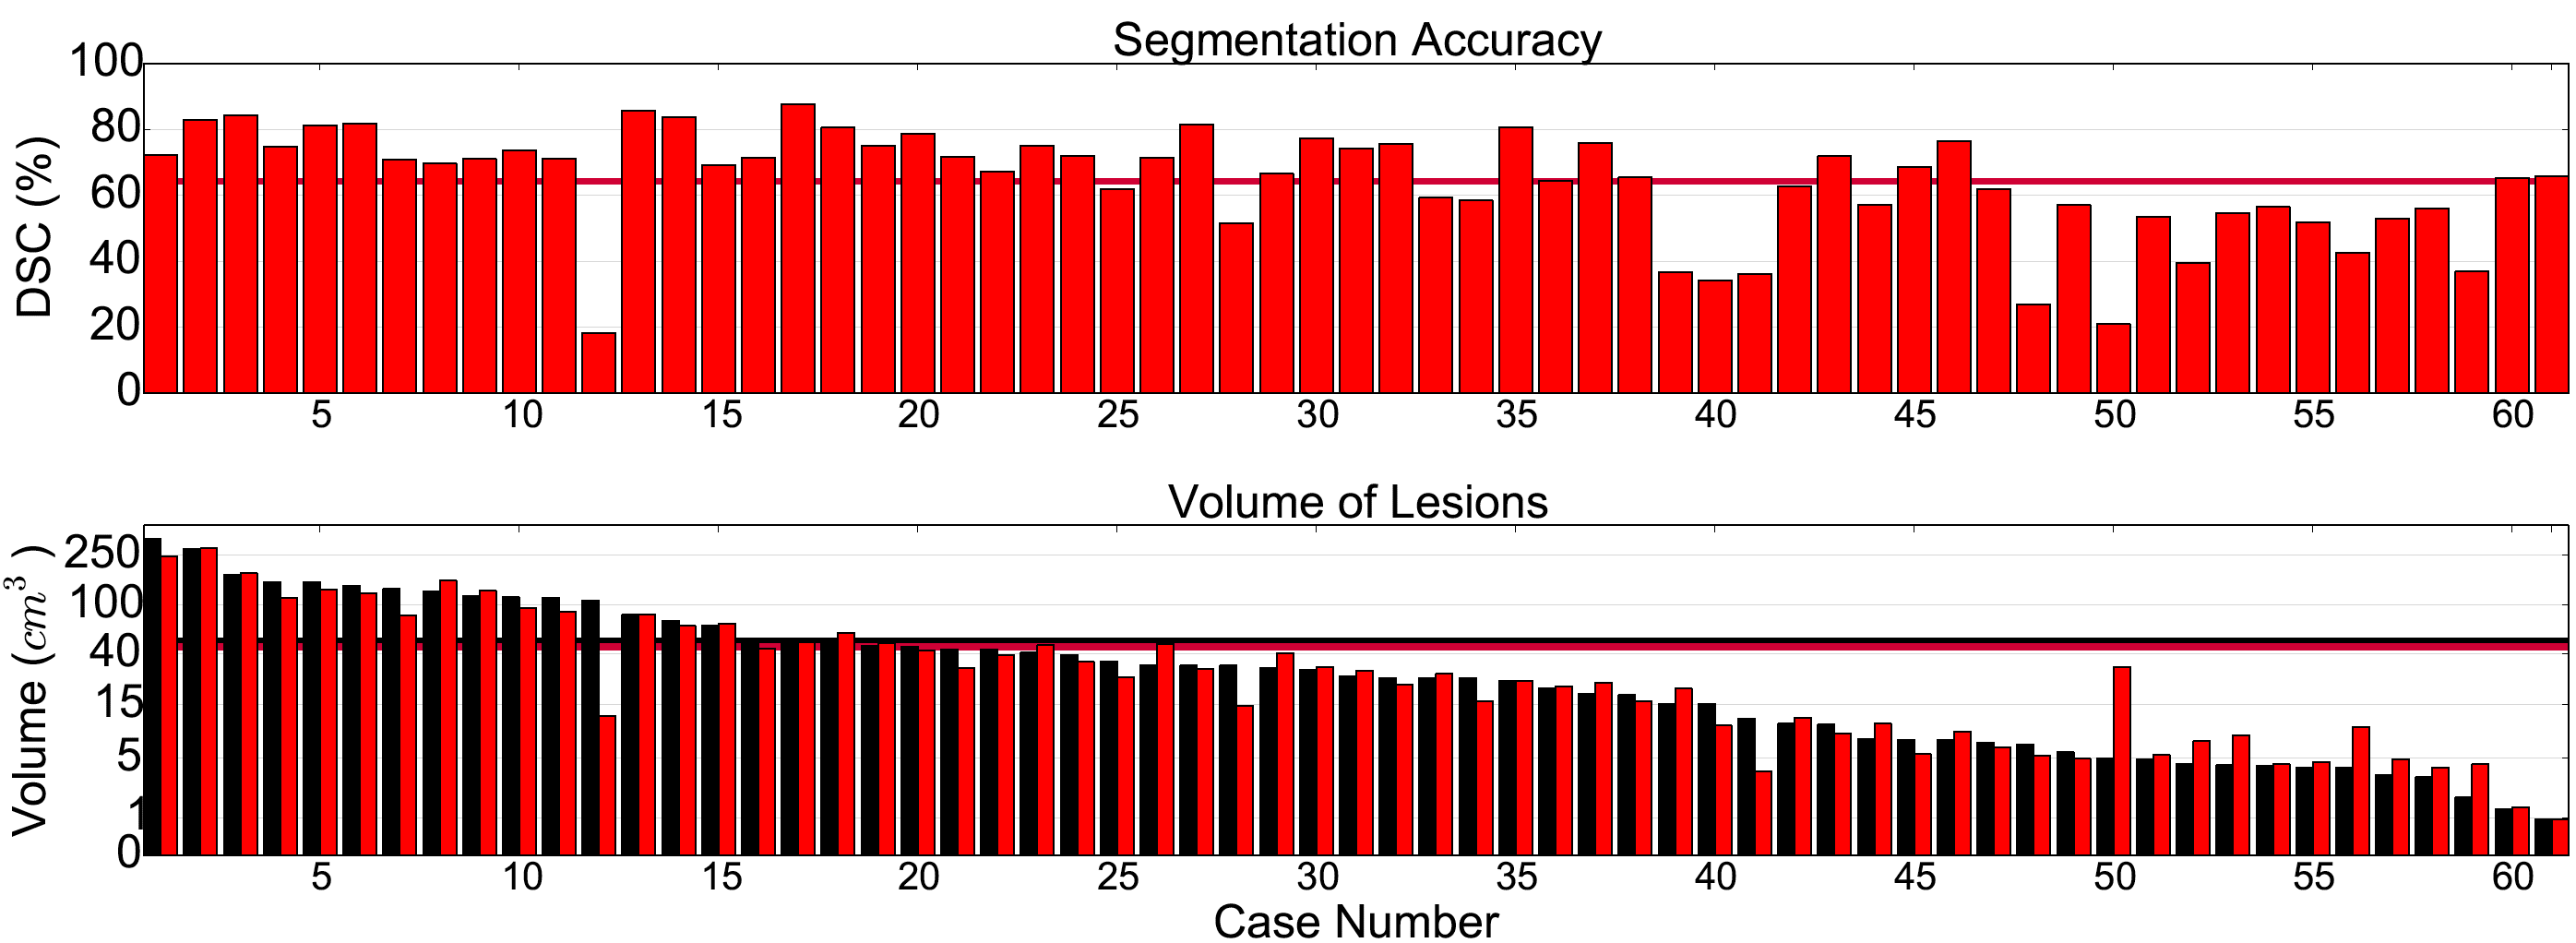
\includegraphics[clip=true, trim=0pt 0pt 0pt 0pt, width=1.0\textwidth]{figures/evaluationSection/tbi/resultsVsLesionVolume/tbiAccuracyJournal_nonReg.png}
\end{subfigure}
\vspace{-0pt} %takes away some white space before the caption
\caption{(Top) DSC achieved by our ensemble of three networks on each of the 61 TBI datasets. (Bottom) Manually segmented (black) and predicted lesion volumes (red). Note here the logarithmic scale. Continuous lines represent mean values. The outlying subject 12 presents small TBI lesions, which are successfully segmented, but also vascular ischemia. Because it is the only case in the database with the latter pathology, the networks fail to segment it as such lesion was not seen during training.}
\label{fig:evalTbiAccVsVol}
\vspace{-10pt}
\end{figure}
%\vspace{-1pt} %takes away some white space before figure